\chapter{调试通道总体设计与关键技术}

\section{总体设计}
	VxWorks的集成开发调试环境为Tornado,它使用串口和网口结合的方式来对目标机进行控制和数据传输,而目前对于大多数的设备而言都已经抛弃了串口,很多用于军事上的嵌入式设备都是专用设备,没有联网的需求,并不会配备网口,但是对于设备上产生的各种调试信息、日志信息都需要传输到我们的windows PC上来进行一个事后分析工作,因此我们需要设计一个新的调试通道来满足这些信息的传输要求,我们本次设计一个基于USB口转串口的底层驱动来实现该调试通道。
	调试通道的总体结构如\autoref{fig:debug-system-diagram}所示。
\begin{figure}[!h]
\centering
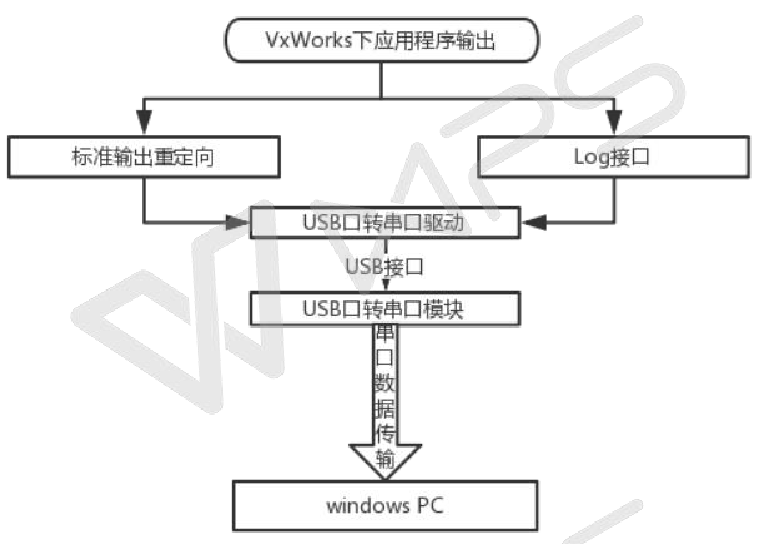
\includegraphics[width=.9\textwidth]{./graphics/debug-system-diagram.pdf}
\caption{调试通道整体结构图}\label{fig:debug-system-diagram}
\end{figure}
	
	整个调试通道主要分为两个模块:应用层的接口模块、USB口转串口模块。
	
	提供给应用层的接口模块负责将系统应用层的输出通过我们的USB口转串口驱动程序传输到windows PC机,输出的形式包括特定内容的格式化的输出和普通的重定向的输出,格式化的输出我们会使用自定义的Log接口进行格式控制,为此我们设计了一个自定义的Log协议格式,其中的内容包含有调试级别、调试信息所在的文件、调试信息所处的行号、输出该条调试信息的时间等;重定向的输出包括RTP模式下的重定向和task模式下的重定向,VxWorks中对于这两种模式需要使用不同的重定向方式。
	
	USB口转串口模块用于在VxWorks上实现一个USB口转串口驱动程序,负责将上层应用的信息传输到windows PC,包括一个特定需求的驱动程序的实现和一个普通的驱动程序的实现。特殊需求的驱动程序相对于普通的驱动程序而言在流程和结构上进行了修改,以使其达到特定的要求,具体的实现我们会在第三节进行介绍。两种实现方式中都会包含有驱动程序加载、卸载模块,设备的打开、关闭、读、写、控制模块。同时在驱动程序中还需要一个数据的管理模块,我们会使用循环缓冲区来管理数据。


\section{关键技术}

\subsection{VxWorks驱动开发}
	
	在VxWorks当中使用I/O子系统来管理设备驱动,I/O 子系统在整个VxWorks当中起着承上启下的作用,各种类型的设备都必须要向I/O子系统进行注册才能够被内核访问,I/O子系统在VxWorks当中的作用是维护系统设备表、系统驱动表、系统文件描述符表\cite{VxWorks内核解读}\cite{曹桂平2011VxWorks}。设备驱动在VxWorks中就靠这三个数据结构来进行管理,所以对于设备驱动而言非常重要。设备驱动程序初始化时会对硬件完成初始化的配置,同时会向I/O子系统注册自己,注册之后I/O子系统才能找到该驱动。

\subsubsection{VxWorks I/O 系统}
	通常操作系统为了平台的无关性都会为应用程序提供一套标准的接口,VxWorks也不例外,它为应用层的提供了接口函数有creat()、open()、unlink()、remove()、close()、rename()、read()、write()、ioctl()、lseek()、readv()、writev()等\cite{陈洋2007VxWorks}\cite{Wu2008Implementation}\cite{Zhang2010Design},我们将其称作为标准I/O 库。
	这样就可以在对应用层的程序进行开发和移植的时候使用同一套接口,大大提高了开发的效率,避免了重复工作,而对于操作系统而言则是通过调整底层驱动或者操作系统中间层来为标准IO提供实现的机制。在Mac OS、Linux、或Windows当中会把这套接口以标准库的形式呈现,但是在VxWorks中它们是由系统的内核实现的,直接以内核文件的形式提供的,它们都位于ioLib.c文件下\cite{VxWorks内核解读}。
	
	VxWorks与通用操作系统的一个很大的不同点是它不会区分用户态和内核态,所有的内核函数都可以不加限制的由用户程序直接进行调用,这样就减少了中断转入内核态再继续执行这一个过程,这对于强实时性系统而言极为重要,因为这样减少了时间开销,但是这样减少了使用权限上的限制,为内核带来了不安全性,极易导致内核的崩溃,所以VxWorks系统上应用程序的开发和使用对开发人员的要求比较高。
		
	I/O调用结构如\autoref{fig:I/O调用}所示。
	\begin{figure}[!h]
\centering
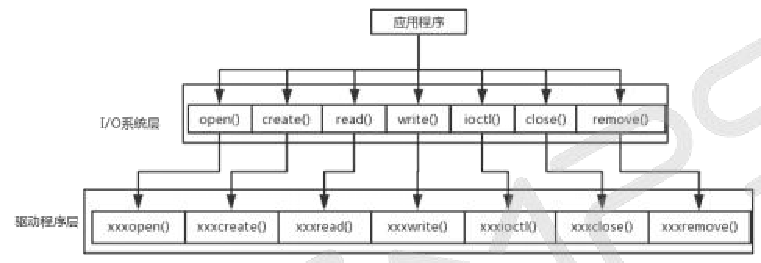
\includegraphics[width=1.0\textwidth]{./graphics/IOCall.pdf}
\caption{I/O调用}\label{fig:I/O调用}
\end{figure}

	
\subsubsection{系统设备表}
	系统设备表是VxWorks中为了管理系统上的所有设备而使用的一个链表。系统设备表在系统中的连接方式如\autoref{fig:VxWorks系统设备示意图}所示。wind内核规定每一个设备都必须使用一个DEV\_ HDR的结构来表示该设备,该结构中只包含有三个成员:一个设备链表节点;一个设备驱动号;一个指向设备名的指针。
	其定义如\autoref{fig:DEVHDR} 所示。

\begin{figure}[!h]
\centering
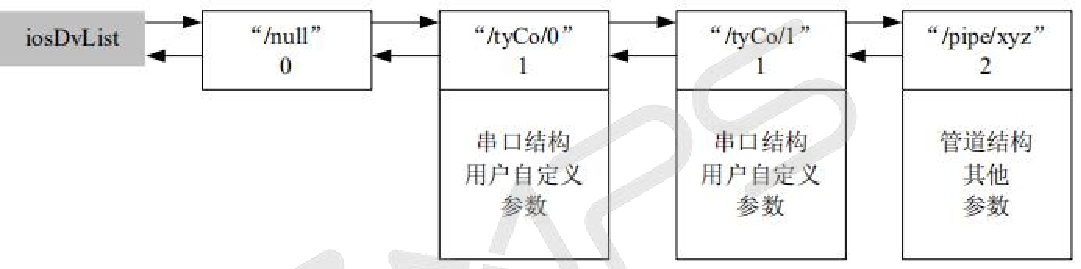
\includegraphics[width=1.0\textwidth]{./graphics/vxworks-device-link.pdf}
\caption{VxWorks系统设备示意图}\label{fig:VxWorks系统设备示意图}
\end{figure}
	
\begin{figure}[!h]
\centering
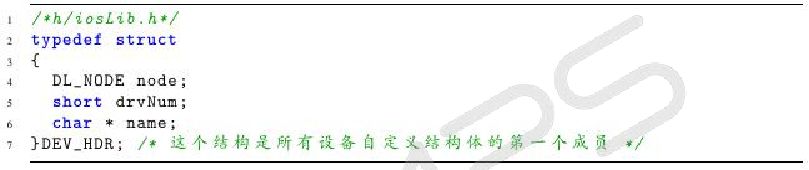
\includegraphics[width=1.0\textwidth]{./graphics/DEVHDR.pdf}
\caption{DEV\_ HDR结构体}\label{fig:DEVHDR}
\end{figure}

VxWorks系统提供了一个设备的注册函数iosDevAdd( DEV\_ HDR *pDevHdr, char *name, int drvnum),该函数用来将一个设备添加到系统设备表当中,系统设备表在每次添加设备时就会增加一个节点,删除设备时就会减少一个节点,一个设备添加到系统之后,就可以使用open()函数通过文件名对所有设备链表中的表项进行匹配,匹配成功之后就可以实现文件与设备的连接\cite{刘小军2008基于},之后就可以使用相对应的注册的设备驱动进行其他的文件操作。VxWorks中使用最佳匹配的方式进行设备名匹配。

\subsubsection{系统驱动表}	
	系统驱动表用于管理当前注册到I/O子系统下的所有驱动程序,所管理的驱动既可以是直接驱动硬件工作的驱动层,也可以是驱动的中间层\cite{VxWorks内核解读}。
	
	VxWorks中使用数组来实现系统驱动表,表中的每一个表项都是一个 DRV\_ ENTRY 类型的结构,该结构定义在内核的头文件iosLibP.h当中,其定义如\autoref{fig:DEVENTRY}所示。
	
\begin{figure}[!h]
\centering
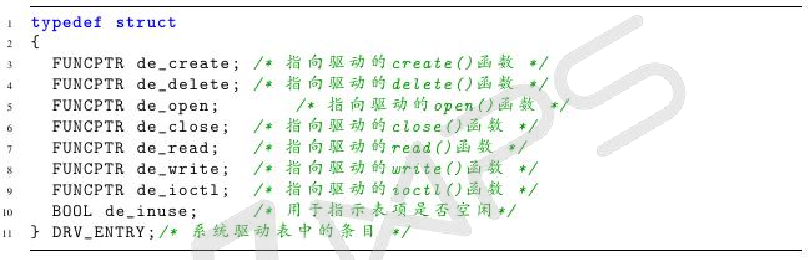
\includegraphics[width=1.0\textwidth]{./graphics/DEVENTRY.pdf}
\caption{DEV\_ ENTRY结构体}\label{fig:DEVENTRY}
\end{figure}

DEV\_ ENTRY结构体类型当中的成员都是结构体指针,每一个成员指向驱动程序中的一个用于完成特定功能的实际模块,这些模块的功能 要符合IO系统预定义好的标准,要与用户层提供标准函数接口一一对应\cite{VxWorks内核解读}\cite{VxWorksDriverAPI}\cite{Wind2003VxWorks}。DEV\_ ENTRY结构中还有一个相对特殊的成员 de\_ inuse 若该成员空闲则表示该表项未被使用。这个结构体中的函数指针实际指向的内容由驱动调用iosDrvInstall()函数来提供。 该函数的作用就是将驱动注册到系统驱动表当中,并根据注册的内容来填充DRV\_ ENTRY表项的内容。


\subsubsection{系统文件描述符表}
	系统描述符表用于管理当前系统打开的所有文件描述符,在底层也是用一个数组来实现的。文件描述符表的表项索引会被当做是文件描述符的ID(即open()返回值)来使用,系统中每次使用open()调用就会占用一个系统文件描述符的表项。VxWorks中的标准输入、标准输出、标准错误输出虽然使用 0,1,2 三个文件描述符来表示,但是它在底层的实现上可能并不是占用了三个表项,而是只占用一个表项,即三个文件描述符指向同一个表项\cite{VxWorks内核解读}\cite{An2003Implementation},这一点是需要注意的。
		
	
系统文件描述符表中每一个表项都使用 FD\_ ENTRY 这个结构来表示,这个结构定义在内核的头文件iosLibP.h 中,其定义如\autoref{fig:FDENTRY}所示。


\begin{figure}[!h]
\centering
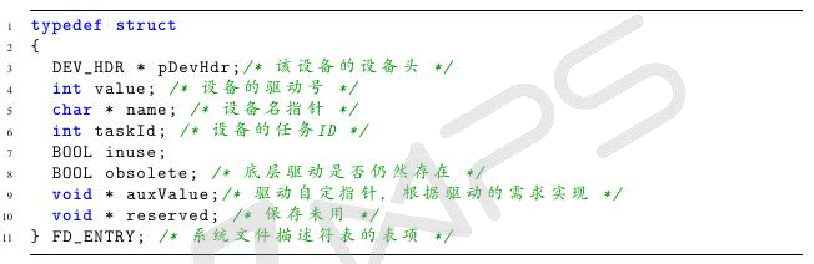
\includegraphics[width=1.0\textwidth]{./graphics/FDENTRY.pdf}
\caption{FD\_ ENTRY结构体}\label{fig:FDENTRY}
\end{figure}


用户的应用程序每次使用open()系统调用系统文件描述符表中就会增加一个有效表项,该表项的FD\_ ENTRY结构体会根据open()调用的内容来进行填充,每一个文件能够进行的open()调用是有限制的,每个驱动的FD\_ ENTRY结构数组满了之后就无法再对这个设备进行open()操作,此时 open()函数将会失败返回\cite{VxWorks内核解读}。系统会在表中的索引偏移 3 之后找一个最先找到的未使用的id作为文件描述符返回给用户,之后用户对设备的其他操作只需要使用这个文件描述符作为文件句柄即可。	
	
\subsection{VxWorks 中的通信机制}
	
	任务间的通信机制用于协调多个任务之间的活动,在我们的USB口转串口驱动程序当中需要使用任务间的通信机制来确保对驱动缓冲区的中的数据正确、有序的读写,VxWorks内核当中为我们提供了丰富的任务间通信机制,包括共享内存、信号量、消息队列、管道、信号、Sockets等。我们主要介绍一下VxWorks任务中使用较多的信号量、消息队列和管道这三种机制,它们在本质上都是使用的共享物理内存机制,只是这块共享的内存不是由用户进行管理,而是交由内核进行管理的,这种实现机制可以使任务间通信安全有序的进行\cite{胡明民2012基于实时操作系统}\cite{冯云贺2014基于}。

\begin{enumerate}
	\item \textbf{信号量}
	
	作为一种在程序的设计当中最常出现的通信机制,信号量的主要作用是线程间的互斥和同步。VxWorks中为程序提供POSIX信号量的同时设计了专门的Wind信号量,POSIX信号量的使用主要是为了方便程序的移植。
	和POSIX信号量的不同之处在于,VxWorks中对Wind信号量进行了高度的优化,使得其更适用于实时操作系统,能够更快的实现任务间通信。VxWorks中信号量是一个指向SEMAPHORE类型的结构指针,提供了二进制信号量、互斥信号量、计数信号量三种类型的信号量机制,他们适用于解决不同类型的问题。
	
	二进制信号量是最快、最通用的信号量,既可以用于同步也可以用于资源计数。wind的二进制信号量所需系统开销最少,适用于高性能的需求。二进制信号量在资源可用时标记为FULL,在资源不可用时标记为EMPTY。在VxWorks中二进制信号量使用函数semBCreate()来创建,二进制信号量的提取和释放过程如\autoref{fig:二进制信号量的提取与释放过程} 所示。

\begin{figure}[h]
\centering
  \begin{subfigure}[b]{1.0\textwidth}
  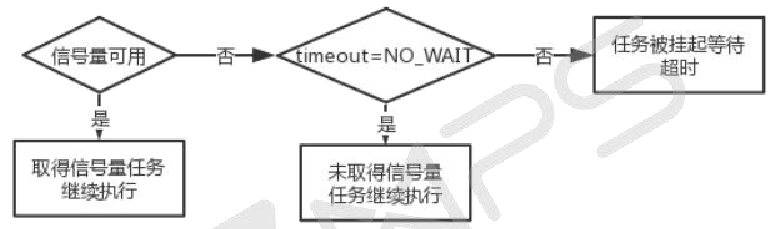
\includegraphics[width=\textwidth]{./graphics/erjinzhiTiQu.pdf}
  \caption{提取信号量}\label{fig:cp2102Front}
  \end{subfigure}
  ~
  \begin{subfigure}[b]{1.0\textwidth}
  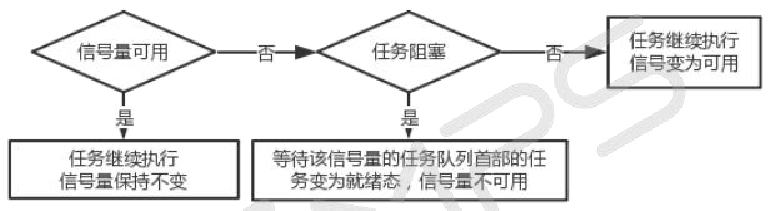
\includegraphics[width=\textwidth]{./graphics/erjinzhiShiFang.pdf}
  \caption{释放信号量}\label{fig:cp2102Rear}
  \end{subfigure}
\caption{二进制信号量的提取与释放过程}\label{fig:二进制信号量的提取与释放过程}
\end{figure}

	
	互斥信号量可以看做是一种特殊的二进制信号量(资源数为1),它优化了互斥、优先级继承、删除安全等问题,这使得它能够更好的服务于任务间的互斥需求;互斥信号量的基本行为和二进制信号量是一致的,但是互斥信号量只能够用于互斥,不能够用于同步,该信号量只能够由获得的该信号量的进程来进行释放,不能够由其它的进程进行释放。它使用SEM\_ INVERSION\_ SAFE和SEM\_ Q\_ PRIORITY选项来使得该信号量能继承优先级算法,以此解决优先级的倒置问题;使用SEM\_ DELETE\_ SAFE选项来解决删除安全问题,在VxWorks中互斥信号量使用系统提供的semMCreate()函数来创建;
	
	资源计数信号量也是一种特殊的二进制信号量(资源数较多),它会跟踪信号量增加、删除的次数,每次释放一个信号量,内部的计数器就会执行加一操作,每次提取一个信号量,内部的计数器就会执行减一操作,当计数器为0时,表示没有可供使用的资源,此时提取信号量的操作就会被阻塞,在VxWorks中资源计数信号量使用系统提供的semCCreate()函数来创建。
	
三种信号量的释放操作都是使用semGive()函数;提取操作都是使用semTake()函数,在提取信号量是我们可以选择是否允许超时,超时可以作为解决阻塞的一种方法。

	
	\item \textbf{消息队列}
	
	消息队列是一种在消息传输的过程中保存消息的容器,它给互相合作的任务间通信提供了一种机制。如\autoref{fig:消息队列}是消息队列实现任务间通信的一种方式。
	和信号量类似,VxWorks中支持POSIX消息队列,主要是为了方便移植和程序的兼容,同时VxWorks也设计了专门用于Wind的消息队列,位于msgQLib文件当中。VxWorks中提供函数msgQCreate()来创建一个消息队列;msgQDelete()用于删除一个消息队列;msgSend()用于向消息队列中发送一个消息;masgQReveice()用于从消息队列中提取一个消息。
	
	在wind中消息队列是使用结构数组来实现的,在创建消息队列时必须指定一个消息的最大长度和队列中能够容纳的消息数量,这就使得其在任务间传递较多信息时存在的很大的局限性\cite{冯云贺2014基于}。
	
\begin{figure}[!h]
\centering
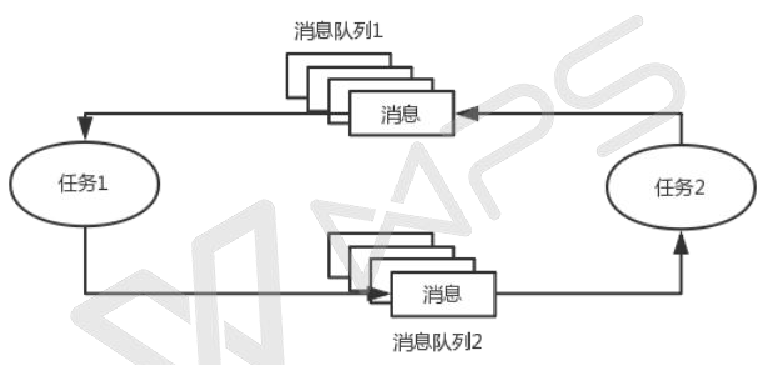
\includegraphics[width=0.9\textwidth]{./graphics/messageQueue.pdf}
\caption{消息队列实现全双工通信}\label{fig:消息队列}
\end{figure}	
				
	
	
	\item \textbf{管道}
	
	管道也是一种基本的进程间通信机制,包括命名管道和匿名管道。VxWorks内核当中使用环形队列的方式来实现管道,管道提供了比消息队列更流畅的信息传递机制,可以像文件一样进行读写。命名管道具有一个与之关联的路径名,因此任何的进程间都可以用它进行通信,命名管道是双工的数据可以双向流动;非命名管道一般用于父子或兄弟进程间通信,非命名管道是半双工的,数据只能向一个方向流动。
\end{enumerate}\\		
\textbf{任务间特殊的通信机制--信号:} 信号通常用于通知一个进程发生了异步事件,也被称为软中断。通常收到信号的进程通常可以选择三种方式来处理:一是使用一个信号处理函数处理;二是选择忽略该信号;三是使用系统默认的处理方式处理。
Wind内核同时支持UNIX BSD风格的信号和POSIX 信号,但是Vxworks中的信号处理机制有些特别之处,对于SIGKILL,SIGSTOP这类的信号,在通用操作系统上是不允许用户修改其默认处理函数的,但是在 VxWorks 操作系统中可以对任何信号的处理函数都可以进行更换的。



\subsection{USB技术}
	USB(Universial Serial Bus)作为PC领域的最新型的接口技术,目前已被各个PC厂家所支持,并且在各类外设当中都广泛的采用USB接口。USB的开发技术也已经很成熟,通用串行总线开发者论坛(USB Implementers Forum,USB IF)目前制定了三种USB接口标准:USB1.1,USB2.0和USB3.0。USB采用菊花链的形式连接所有的设备,最多可以连接127个设备,USB的总线拓扑结构如\autoref{fig:USB体系结构}所示
\begin{figure}[!h]
\centering
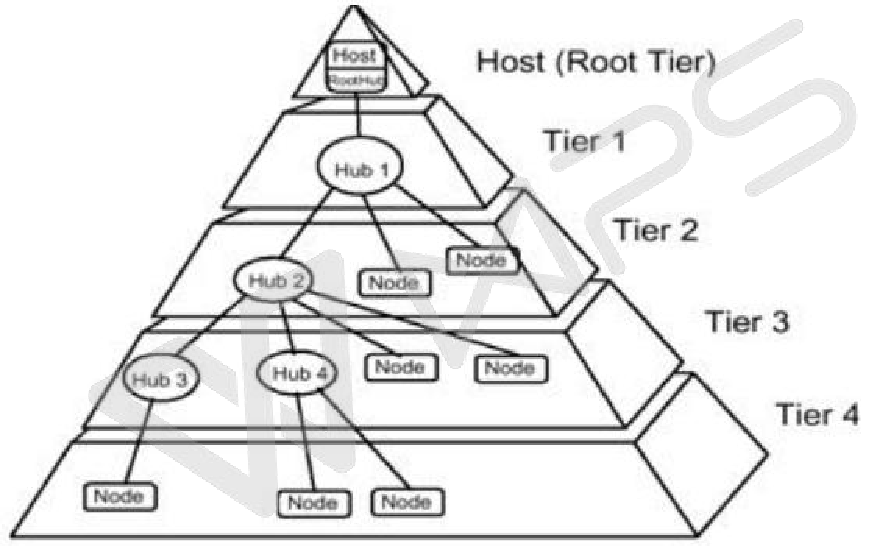
\includegraphics[width=1.0\textwidth]{./graphics/usb-structure.pdf}
\caption{USB总线拓扑结构}\label{fig:USB体系结构}
\end{figure}


USB的体系结构由三个部分组成,分别是USB主机(Host)、USB集线器(Hub)、USB设备(Device)。其中我们需要了解的关键部分是USB主机和USB设备。
	
\begin{enumerate}
\item \textbf{USB主机}\\
	USB主机是USB体系中的核心,且系统中只允许一个USB主机存在。USB主机上的USB接口是USB主控制器,其控制着总线上所有USB设备数据通信。对于USB的体系结构而言,其数据的传输都是USB主机端发起的,非主机端(设备端)只能够被动的进行响应。USB主机需要完成的功能包括检测设备的热插拔、管理主机和设备之间的信息(控制和数据)流\cite{李雪红2004USB}\cite{莫宏伟2001USB}。



\item \textbf{USB设备}

	USB设备指的是提供具体功能的而外部USB设备,是相对USB主机而言的,它们受USB主机的控制,只能对主机的请求进行被动响应。USB主机端会在检测到USB设备的动作之后会通过默认管道和USB设备进行通信,对其进行必要的初始化配置,并给设备提供适合的驱动程序(如果有的话),一个USB设备会通常会有很多的属性,它会通过这些属性来完成主机的配置要求。一些USB设备的属性如下:
	\begin{itemize}
	\item \textbf{描述符(Descriptor)属性}\\
	描述符是USB协议中定义的一套用来描述USB设备的功能和属性的固定结构,我们可以通过描述符了解设备的各种属性和,描述符又分为设备描述符、配置描述符、接口描述符、端点描述符、字符串描述符\cite{张杰2008基于}\cite{边海龙2004USB}除此之外,设备还可以提供自己专用的描述符,分为设备类描述符和供应商自定义描述符,我们使用的USB口转串口设备就不属于一个标准的USB设备,它会为我们提供供应商自定义的描述符,我们之后需要用它来对设备进行识别。
	
	\item \textbf{类(Class)属性}\\
	由于USB协议支持许多的外围设备,而这些设备又可以根据功能来分成一些相近的类,如打印机类、键盘类等。这样主机端只需要提供类驱动程序便可以驱动大多数的USB设备,而不需要再为每一个设备提供一个完整的驱动程序。这大大的方便的设备的制造商。他们的设备只需要符合某一类的驱动,就可以使用该类驱动程序来驱动其设备,之后只需要实现简单的包含有设备特性的客户端驱动即可,不需要再实现复杂的底层驱动程序\cite{李雪红2004USB}。	
	
	\item \textbf{功能(Function)/接口(Interface)属性}\\
	功能或接口是USB协议中定义的设备的某种能力,Function是从功能角度来说的,从设备的角度来说,被称为Interface。一个设备可以拥有几个接口,每一个接口负责完成设备的一个特定的功能,并且这个接口的功能是可以替换的,当USB设备处于可配置状态的时候能够通过控制命令来改变某一个接口的功能,对于USB设备的每一个接口都必须要有一个接口描述符来描述。
	
	\item \textbf{端点(Endpoint)属性}\\
	端点是USB设备与USB主机逻辑上的通信流的终点,每个设备都拥有一个可独立进行操作的端点集合,且每个端点在使用时都要先初始化其数据传输方向(IN/OUT),即使端点号相同但是传输方向不同的通信点也是不同的端点\cite{李雪红2004USB}。
	
	\item \textbf{管道}\\
	管道可以看做是设备上的一个端点和主机上的软件的联合体,设备和主机间的数据传输要基于管道进行。在USB的通信过程中首先要建立一个管道才能够进行数据的传输,USB设备在和主机通信时都会建立一个默认的管道,这个管道对应的端点是默认端点0,之后需要自己使用其它的端点来建立我们的数据传输过程中需要使用的输入或输出管道。在我们的USB口转串口驱动中会为每一个设备建立两个管道,一个批量输出管道和一个批量输入管道。
	
	\item \textbf{设备地址}\\
	设备地址用于区分USB系统中的一个USB设备的特殊标识,设备地址会在设备初始化之后由主机进行分配且是唯一的。设备地址单元共有7bit,其中地址0是缺省地址,在设备初始化的时候使用,理论上系统可以区分127个USB设备\cite{李雪红2004USB}。
	\end{itemize}	
	
\end{enumerate}



\noindent USB规范规定了USB主从设备之间的四种传输方式,每种方式有各自的用途\cite{USB总线接口开发指南}:
\begin{itemize}
\item \hei{控制传输}:控制传输USB传输方式中最重要、最复杂的一种,它适用于少量、对时间和速率无要求的场合,一个USB设备插入主机之后就是使用这种传输方式来读取设备的地址和描述符等信息。所有的设备都会在其0号端点的缺省管道当中支持控制传输\cite{张杰2008基于}。
\item \hei{批量传输}:批量传输有两种最基本的事物类型:BULK\_ IN和BULK\_ OUT,其主要用于处理对数据传输速率不是很高的情况,批量传输使我们的USB口转串口设备所使用的主要传输传输方式,每次有数据需要传输时我们都会构建一个IRP使用批量传输将其传出或传入。
\item \hei{中断传输}:中断传输也有两种基本的事务:IN和OUT,其主要是为那些要快速实现主机和设备的交互,但是数据量很小、对服务时间有要求的情况而准备的。
\item \hei{等时传输}:等时传输也是由基本的IN和OUT两种事务组成,主要用于处理大量、恒速、对时间周期有要求的数据。等时传输只有全速和高速设备才支持,低速设备不支持\cite{张杰2008基于}。
\end{itemize}


	

\section{本章小结}
	本章重点介绍了本次的VxWorks调试通道的整体架构,并介绍了介绍了各个部分的设计方案,最后介绍了在本次的设计当中所需要使用关键技术和所需了解的重要知识,主要包括VxWorks下的驱动开发必须的结构、驱动中所需使用的VxWorks的通信机制、缓冲区技术、USB技术。下面将要讨论VxWorks下的调试通道的详细的设计细节和具体的实际机制。

























